\documentclass[12pt]{article} %***
\usepackage[sectionbib]{natbib}
\usepackage{array,epsfig,fancyheadings,rotating}
%\usepackage[]{hyperref}  %<----modified by Ivan
%%%%%%%%%%%%%%%%%%%%%%%%%%%%%%%%%%%%
\usepackage{sectsty, secdot}
%\sectionfont{\fontsize{12}{15}\selectfont}
\sectionfont{\fontsize{12}{14pt plus.8pt minus .6pt}\selectfont}
\renewcommand{\theequation}{\thesection\arabic{equation}}
\subsectionfont{\fontsize{12}{14pt plus.8pt minus .6pt}\selectfont}
%%%%%%%%%%%%%%%%%%%%%%%%%%%%%%%%%%%%%%%%%%%%%%%%%%%%%%%%%%%%%%%%%%%%%%%%%%%%%%%%%%%%%%%%

\textwidth=36pc
\textheight=49pc
\oddsidemargin=1pc
\evensidemargin=1pc
\headsep=15pt
\topmargin=.6cm
\parindent=1.7pc
\parskip=0pt

\usepackage{amsmath}
\usepackage{amssymb}
\usepackage{amsfonts}
\usepackage{multirow}
\usepackage{amsthm}
\usepackage{todonotes}
\usepackage{mathtools}
\usepackage{subcaption}
\usepackage{color}
\usepackage{cite}

\usepackage{xr}
\externaldocument{hyperparam-theory-appendix}


\setcounter{page}{1}
\newtheorem{theorem}{Theorem}
\newtheorem{lemma}{Lemma}
\newtheorem{corollary}{Corollary}
\newtheorem{proposition}{Proposition}
\theoremstyle{definition}
\newtheorem{definition}{Definition}
%\newtheorem{proof}{Proof}
\newtheorem{example}{Example}
\newtheorem{remark}{Remark}
\newtheorem{condition}{Condition}
\newtheorem{assump}{Assumption}
\DeclareMathOperator{\diag}{diag}
\DeclareMathOperator{\spann}{span}
\newcommand{\textred}[1]{\textcolor{red}{#1}}
\pagestyle{fancy}

%%%%%%%%%%%%%%%%%%%%%%%%%%%%%%%%%%%%%%%%%%%%%%%%%%%%%%%%%%%%%%%%%%%%%%%%%%%%%%%%%%%%%%%%%%%%%%%%%%%%%%%%%%%%%%%%%%%%%%%%%%%%
\pagestyle{fancy}
\def\n{\noindent}
\lhead[\fancyplain{} \leftmark]{}
\chead[]{}
\rhead[]{\fancyplain{}\rightmark}
\cfoot{}
%\headrulewidth=0pt  %<-modified by Ivan

%%%%%%%%%%%%%%%%%%%%%%%%%%%%%%%%%%%%%%%%%%%%%%%%%%%%%%%%%%%%%%%%%%%%%%%%%%%%%%%%%%%%%%%%%%%%%%%%%%%%%%%%%%%%%%%%%%%%%%%%%%%%

\DeclareMathOperator*{\argmin}{arg\,min}

%%%%%%%%%%%%%%%%%%%%%%%%%%%%%%%%%%%%%%%%%%%%%%%%%%%%%%%%%%%%%%%%%%%%%%%%%%%%%%%%%%%%%%%%%%%%%%%%%%%%%%%%%%%%%%%%%%%%%%%%%%%%

\cfoot{\thepage}

\begin{document}

%%%%%%%%%%%%%%%%%%%%%%%%%%%%%%%%%%%%%%%%%%%%%%%%%%%%%%%%%%%%%%%%%%%%%%%%%%%%%%%%%%%%%%%%%%%%%%%%%%%%%%%%%%%%%%%%%%%%%%%%%%%%
%%%%%%%%%%%%%%%%%%%%%%%%%%%%%%%%%%%%%%%%%%%%%%%%%%%%%%%%%%%%%%%%%%%%%%%%%%%%%%%%%%%%%%%%%%%%%%%%%%%%%%%%%%%%%%%%%%%%%%%%%%%%

\renewcommand{\baselinestretch}{2}

\markright{ \hbox{\footnotesize\rm Statistica Sinica
%{\footnotesize\bf 24} (201?), 000-000
}\hfill\\[-13pt]
\hbox{\footnotesize\rm
%\href{http://dx.doi.org/10.5705/ss.20??.???}{doi:http://dx.doi.org/10.5705/ss.20??.???}
}\hfill }

\markboth{\hfill{\footnotesize\rm Jean Feng and Noah Simon} \hfill}
{\hfill {\footnotesize\rm Hyper-parameter selection via split-sample validation} \hfill}

\renewcommand{\thefootnote}{}
$\ $\par

%%%%%%%%%%%%%%%%%%%%%%%%%%%%%%%%%%%%%%%%%%%%%%%%%%%%%%%%%%%%%%%%%%%%%%%%%%%%%%%%%%%%%%%%%%%%%%%%%%%%%%%%%%%%%%%%%%%%%%%%%%%%

\fontsize{12}{14pt plus.8pt minus .6pt}\selectfont \vspace{0.8pc}
\centerline{\large\bf An analysis of the cost of hyper-parameter selection via split-}
\vspace{2pt} \centerline{\large\bf sample validation, with applications to penalized regression}
\vspace{.4cm} \centerline{Jean Feng, Noah Simon} \vspace{.4cm} \centerline{\it
Department of Biostatistics, University of Washington} \vspace{.55cm} \fontsize{9}{11.5pt plus.8pt minus
.6pt}\selectfont

%%%%%%%%%%%%%%%%%%%%%%%%%%%%%%%%%%%%%%%%%%%%%%%%%%%%%%%%%%%%%%%%%%%%%%%%%%%%%%%%%%%%%%%%%%%%%%%%%%%%%%%%%%%%%%%%%%%%%%%%%%%%

\begin{quotation}
\noindent {\it Abstract:}
In the regression setting, given a set of hyper-parameters, a model-estimation procedure constructs a model from training data. The optimal hyper-parameters that minimize generalization error of the model are usually unknown. In practice they are often estimated using split-sample validation. Up to now, there is an open question regarding how the generalization error of the selected model grows with the number of hyper-parameters to be estimated. To answer this question, we establish finite-sample oracle inequalities for selection based on a single training/test split and based on cross-validation. We show that if the model-estimation procedures are smoothly parameterized by the hyper-parameters, the error incurred from tuning hyper-parameters shrinks at nearly a parametric rate. Hence for semi- and non-parametric model-estimation procedures with a fixed number of hyper-parameters, this additional error is negligible. For parametric model-estimation procedures, adding a hyper-parameter is roughly equivalent to adding a parameter to the model itself. In addition, we specialize these ideas for penalized regression problems with multiple penalty parameters. We establish that the fitted models are Lipschitz in the penalty parameters and thus our oracle inequalities apply. This result encourages development of regularization methods with many penalty parameters.
\vspace{9pt}

\noindent {\it Key words and phrases:}
Cross-validation, Regression, Regularization.
\par
\end{quotation}\par

\def\thefigure{\arabic{figure}}
\def\thetable{\arabic{table}}

\renewcommand{\theequation}{\thesection.\arabic{equation}}



\fontsize{12}{14pt plus.8pt minus .6pt}\selectfont

\setcounter{section}{1} %***
\setcounter{equation}{0} %-1

\section{Introduction}

%JF wow this paper's english can really use some level-upping. some paragraphs also don't flow.
%JF clean up notation - bold symbols appropriately too!

Per the usual regression framework, suppose we observe response $y \in \mathbb{R}$ and predictors $\boldsymbol {x} \in \mathbb{R}^p$. Suppose $y$ is generated by a true model $g^*$ plus random error $\epsilon$ with mean zero, as follows
\begin{equation}
\label{true_model}
y = g^*(\boldsymbol x) + \epsilon.
\end{equation}
Our goal is to estimate $g^*$.
Many model-estimation procedures can be formulated as selecting a model from some function class $\mathcal{G}$ given training data $T$ and $J$-dimensional hyper-parameter vector $\boldsymbol{\lambda}$. For example, in penalized regression problems, the fitted model can be expressed as the minimizer of the penalized training criterion
\begin{equation}
\label{eq:intro_pen_reg}
\hat{g}(\boldsymbol \lambda | T) = \argmin_{g\in \mathcal{G}} \sum_{(\boldsymbol{x}_i, y_i) \in T} \left (y_i -  g(\boldsymbol{x}_i) \right )^2 + \sum_{j=1}^J \lambda_j P_j(g),
\end{equation}
%JF:  I would like to divide by number of obs in T
where $P_j$ are penalty functions and $\lambda_j$ are penalty parameters. As suggested by the notation in \eqref{eq:intro_pen_reg}, the penalty parameters are the hyper-parameters in this model-estimation procedure.

%JF english, man...
Given a set of possible hyper-parameters $\Lambda$, a training dataset $T$, and norm $\|\cdot\|$, there exist oracle hyper-parameters $\tilde{\Lambda} \subseteq \Lambda$ that minimize the difference between the fitted model $\hat{g}\left(\boldsymbol{\lambda|}T\right)$ and the true model:
%JF: is reviewer2 referring to this?
\[
\tilde{\Lambda} = \argmin_{\lambda \in \Lambda} \left\|g^{*} - \hat{g}\left(\boldsymbol{\lambda|}T\right)\right\|^2.
\]
$\tilde{\Lambda}$ is unknown and so a sample-splitting procedure is often used to find a $\hat{\boldsymbol{\lambda}}$ in $\tilde{\Lambda}$.
The basic idea is to fit models on a random partition of the observed data and evaluate their error on the remaining data.
The final hyper-parameters $\hat{\boldsymbol{\lambda}}$ are chosen to minimize the error on this validation set.
For a more complete review of cross-validation, refer to \citet{arlot2010survey}.

The performance of split-sample validation procedures is typically characterized by an oracle inequality that bounds the generalization error of the expected model selected from the validation set procedure. For $\Lambda$ that are finite, oracle inequalities have been established for a single training/validation split \citep{gyorfi2006distribution} and a general cross-validation framework \citep{van2003unified, van2004asymptotic}. To handle $\Lambda$ over a continuous range, one can use entropy-based approaches \citep{lecue2012oracle}.
%JF: I would like to add reasons for why we want to think about a continuous range because people don't typically think about this.

The goal of this paper is to characterize the performance of models when the hyper-parameters are tuned by some split-sample validation procedure. We are particularly interested in an open question raised in \citet{bengio2000gradient}: what is the ``amount of overfitting... when too many hyper-parameters are optimized''? In addition, how many hyper-parameters is ``too many''? In this paper we show that actually a large number of hyper-parameters can be tuned without overfitting. In fact, if an oracle estimator converges at rate $R(n)$, then the number of hyper parameters $J$ can grow at roughly a rate of $J = O_p(nR(n))$ up to log terms without affecting the convergence rate. In practice, for penalized regression, this means that one can propose and tune over much more complex models than are currently often used.

To show these results, we prove that finite-sample oracle inequalities of the form
\begin{equation}
\label{thrm:intro_oracle_ineq}
\left \| g^* - \hat{g} (\hat{\boldsymbol{\lambda}} | T ) \right \|^2
\le
(1+a)
\underbrace{\inf_{\lambda \in \Lambda} \left \| g^* - \hat{g}\left (\boldsymbol{\lambda} \middle | T \right ) \right \|^2}_{\text{Oracle error}}
+ \delta \left(J,n\right)
\end{equation}
%JF: Is review2 referring to this?!
are satisfied with high probability for norm $\| \cdot \|$, constant $a \ge 0$, and remainder $\delta(J,n)$ that depends on the number of tuned hyper-parameters $J$ and the number of samples $n$.
Under the assumption that the model -estimation procedure is \textred{Lipschitz} in the hyper-parameters, we find that $\delta$ scales linearly in $J$.
% be careful here as some reviewer wants to argue log J also happens when you add parameters to the model itself
\textred{So for parametric model-estimation procedures, the additional error from adding a hyper-parameter is roughly equivalent to adding a parameter to the model itself.}
For semi- and non-parametric model-estimation procedures, this error is generally dominated by the oracle error and \textred{the number of hyper-parameters can actually grow without affecting the asymptotic convergence rate}.

In this paper, we also specialize these results to penalized regression models of the form \eqref{eq:intro_pen_reg}. We show that the fitted model is indeed \textred{Lipschitz} in the penalty parameters so our oracle inequalities apply. Again, we find that additional penalty parameters only add a near-parametric error term, which has a negligible effect in semi- and non-parametric settings. This result suggests that the recent interest in combining penalty functions (e.g. elastic net and sparse group lasso \citep{zou2003regression, simon2013sparse}) may have artificially restricted themselves to two-way combinations. Adding more penalties may lead to better models.

During our literature search, we found few theoretical results addressing the relationship between the number of hyper-parameters and generalization error of the selected model. 
Much of the previous work only considered tuning a one-dimensional hyper-parameter over a finite $\Lambda$, proving asymptotic optimality \citep{van2004asymptotic} and finite-sample oracle inequalities \citep{van2003unified, gyorfi2006distribution}. Others have addressed split-sample validation for specific penalized regression problems with a single penalty parameter, such as linear model selection \citep{li1987asymptotic, shao1997asymptotic, golub1979generalized, chetverikov2016cross, chatterjee2015prediction}. Only \citet{lecue2012oracle} has a result that is relevant to answering our question of interest by using techniques from empirical process theory. A potential reason for this dearth of literature is that, historically, tuning multiple hyper-parameters has been computationally difficult. However, there have been many proposals recently for overcoming this computational hurdle \citep{bengio2000gradient, foo2008efficient, snoek2012practical}.
%JF: cite myself? cite more recent snoek?

Section \ref{sec:main_results} presents oracle inequalities for model-estimation procedures that are \textred{Lipschit} in the hyper-parameters.
These results answer our question regarding how the number of hyper-parameters affects the model error.
Section \ref{sec:examples} applies these results to penalized regression models.
Section \ref{sec:simulations} provides a simulation study to support our theoretical results.
Section \ref{sec:discussion} discusses our findings and potential future work.
Oracle inequalities for general model-estimation procedures and proofs for all the results are given in the Supplementary Materials.



\section{Oracle Inequalities} \label{sec:main_results}

In this section, we establish oracle inequalities for models where the hyper-parameters are tuned by a single training/validation split and cross-validation. We first introduce some notation and formalize the model-estimation procedure. 

Let $D^{(n)}$ denote a dataset with $n$ samples from the model \eqref{true_model}. The model-estimation procedure $\hat{g}$ is a set of functions $\{\hat{g}^{(n_T)}\}$ where $\hat{g}^{(n_T)}(\boldsymbol{\lambda} | D^{(n_T)})$ maps hyper-parameter $\boldsymbol{\lambda} \in \Lambda \subseteq \mathbb{R}^J$ and training data $D^{(n_T)}$ to a function in $\mathcal{G}$.

In this \textred{paper}, we focus on model-estimation procedures that are Lipschitz.
\begin{definition}
	\label{def:smooth_funcs}
	Let $\mathcal{G}$ be a function class from $\mathcal{X} \subseteq \mathbb{R}^p \mapsto \mathbb{R}$.
	Let $\Lambda \subseteq \mathbb{R}^J$.
	The operator $g: \Lambda \mapsto \mathcal{F}$ is $C_\Lambda$-Lipschitz in $\boldsymbol{\lambda}$ over $\Lambda$ if there is some function $C_{\Lambda}:\mathcal{X} \mapsto \mathbb{R}^+$ such that for all $\boldsymbol{x} \in \mathcal{X}$,
	\begin{equation}
	\left | g(\boldsymbol \lambda)(\boldsymbol{x}) - g(\boldsymbol \lambda ')(\boldsymbol{x}) \right |
	\le
	C_{\Lambda}(\boldsymbol{x}) \| \boldsymbol \lambda - \boldsymbol \lambda' \|_2 
	\quad
	\forall \boldsymbol \lambda,\boldsymbol \lambda' \in \Lambda.
	\label{eq:smooth_funcs}
	\end{equation}
\end{definition}
%JF: reviewer said reword - is this better?
We believe that many model-estimation procedures satisfy this Lipschitz assumption as procedures that are well-behaved in their hyper-parameters tend to be easier to use and thereby more popular.
For instance, we show in Section \ref{sec:examples} that penalized regression models indeed satisfy this assumption.
In the following sections, we show that the contribution to the error from tuning multiple hyper-parameters for such procedures is roughly parametric.
%JF removing sentences cause it seems repetitive
%Hence for semi- and non-parametric model-estimation procedures, the error from tuning a fixed number of hyper-parameters is negligible.
%Moreover, we can specify an upper bound on the rate at which the number of hyper-parameters can grow without asymptotically increasing the generalization error of the selected model.

\subsection{A Single Training/Validation Split}\label{sec:single}

When tuning hyper-parameters using a single training/validation split, the dataset $D^{(n)}$ is randomly partitioned into a training set $T = (X_T, Y_T)$ and validation set $V = (X_V, Y_V)$ with $n_T$ and $n_V$ observations, respectively.
The selected hyper-parameter $\hat{\boldsymbol{\lambda}}$ is a minimizer of the validation loss
\begin{equation}
\label{eq:train_val_lambda}
\hat{\boldsymbol \lambda} \in \argmin_{\boldsymbol{\lambda} \in\Lambda} \frac{1}{2} \left \| y-\hat{g}^{(n_T)}( \boldsymbol \lambda | T) \right \|_{V}^{2}
\end{equation}
where $\| h \|^2_{V}=\frac{1}{n_V}\sum_{(x_i, y_i)\in V} h^2(x_i, y_i)$ for any function $h$.

We now present a finite-sample oracle inequality for the single training/validation split assuming the model-estimation procedure is Lipschitz.
Our oracle inequality is sharp, i.e. $a=0$ in \eqref{thrm:intro_oracle_ineq}, unlike most other work \citep{gyorfi2006distribution, lecue2012oracle, van2003unified}.
This theorem requires minimal assumptions -- it only requires that $\epsilon$ are sub-gaussian random variables and that the model-estimation procedure is Lipschitz.
The tradeoff is that our oracle inequality only characterizes the fitted model at the validation covariates.
Note that the result below is a special case of Theorem \ref{thrm:train_val_complicated} in Appendix \ref{appendix:train_val}, which applies to general model-estimation procedures.
\begin{theorem}
	\label{thrm:train_val}
	Let $\Lambda=[\lambda_{\min},\lambda_{\max}]^{J}$ where $\Delta_{\lambda} = \lambda_{\max} - \lambda_{\min} \ge 0$.
	% ONLY necessary for the validation set
	Suppose independent random variables $\epsilon_i$ associated with the validation data $(x_i, y_i) \in V$ have expectation zero and are uniformly sub-Gaussian with parameters $b$ and $B$:
	$$
	\max_{i: (x_i, y_i) \in V} B^2 \left ( \mathbb{E} e^{|\epsilon_i|^2/B^2} - 1 \right ) \le b^2.
	$$
	Let training data $T$ be fixed, as well as the covariates of the validation set $X_V$.
	Let the oracle risk be denoted
	\begin{equation}
	\tilde{R}(X_V|T) = \argmin_{\lambda \in \Lambda} \left \| g^*-\hat{g}^{(n_T)}( \boldsymbol{\lambda} | T) \right \|_{V}^{2}.
	\label{eq:tilde_lambda_def}
	\end{equation}
	
	Now suppose there exists a function $C_\Lambda: \mathbb{R}^p \mapsto \mathbb{R}$ such that $\hat g^{(n_T)}(\boldsymbol{\lambda} |D^{(n_T)})$ is $C_\Lambda$-Lipschitz with respect to $\boldsymbol{\lambda}$ over $\Lambda$.
	Then there is a constant $c>0$ only depending on $b$ and $B$ such that for all $\delta$ satisfying
	\begin{equation}
	\delta^{2}
	\ge
	c \left (
	\frac{J \log(\|C_\Lambda(\cdot |T)\|_V \Delta_{\Lambda} n + 1)}{n_{V}}
	\vee 
	\sqrt{\frac{J \log(\|C_\Lambda(\cdot |T)\|_V \Delta_{\Lambda} n + 1)}{n_{V}}
		\tilde{R}(X_V|T)}
	\right )
	\label{thrm:train_val_delta}
	\end{equation}
	we have
	\begin{align}
	Pr\left(
	\left\Vert g^* - \hat{g}^{(n_T)}( \hat{\boldsymbol{\lambda}} | T) \right\Vert _{V}^2 -
	\tilde{R}(X_V|T)
	\ge\delta^2
	\middle | 
	T, X_V
	\right )
	&\le c\exp\left(-\frac{n_{V}\delta^{4}}{c^{2} \tilde{R}(X_V|T)}\right)
	+ c\exp\left(-\frac{n_{V}\delta^{2}}{c^{2}}\right).
	\end{align}
	
\end{theorem}

Theorem \ref{thrm:train_val} states that with high probability, the difference between the true model and the selected model is bounded above by the difference between the true model and the oracle model plus $\delta^2$. Hence $\delta^2$ can be thought of as the error incurred during the hyper-parameter selection process. As seen in \eqref{thrm:train_val_delta}, it is the maximum of two terms: a near-parametric term and the geometric mean of the near-parametric term and the oracle risk. To see this more clearly, we express Theorem \ref{thrm:train_val} using asymptotic notation.
\begin{corollary}
	\label{corr:train_val}
	Under the assumptions given in Theorem \ref{thrm:train_val}, we have
	\begin{align}
	%JF please update
	\left\Vert g^* - \hat{g}^{(n_T)}( \hat{\boldsymbol{\lambda}} | T) \right\Vert _{V}^2 &
	\le \min_{\lambda \in \Lambda} \left\Vert g^* - \hat{g}^{(n_T)}( {\boldsymbol{\lambda}} | T) \right \Vert^2_{V}\\
	& + O_p \left(\frac{J\log (n \|C_\Lambda\|_V \Delta_{\Lambda} )}{n_{V}} \right) 
	\label{eq:asym_train_val_theorem1} \\
	& + O_p \left(
	\sqrt{
		\frac{J \log (n \|C_\Lambda\|_V \Delta_{\Lambda} )}{n_{V}}
		\min_{\lambda \in \Lambda} \left\Vert g^* - \hat{g}^{(n_T)}( {\boldsymbol{\lambda}} | T) \right \Vert^2_{V}
	}
	\right ).
	\label{eq:asym_train_val_theorem2}
	\end{align}
\end{corollary}
From Corollary \ref{corr:train_val}, we see that the risk of the selected model is bounded by the oracle risk, the near-parameteric term \eqref{eq:asym_train_val_theorem1}, and the geometric mean of the two values \eqref{eq:asym_train_val_theorem2}.
%JF reviewer wants us to clarify lasso is different...
We refer to \eqref{eq:asym_train_val_theorem1} as near-parametric because the error term in parametric regression models is usually $O_p(J/n)$, where $J$ is the parameter dimension and $n$ is the number of training samples. Analogously, \eqref{eq:asym_train_val_theorem1} is roughly $O_p(J/n_V)$ modulo a $\log n$ term in the numerator.

In the semi- and non-parametric regression settings, the oracle error usually shrinks at a rate of $O_p(n_T^{-\omega})$ where $\omega \in (0, 1)$, which means that for large $n$, the oracle error will tend to dominate both the error terms. Therefore increasing the number of hyper-parameters for such problems only results in a small increase in the model error. In fact, if the oracle error rate is $O_p(n_T^{-\omega})$, the number of hyper-parameters $J$ can grow at the rate
\begin{equation}
O_p\left (
\frac{n_{V} n_T^{-\omega}}{\log (n \|C_\Lambda\|_V \Delta_{\Lambda})}
\right )
\end{equation}
without affecting the asymptotic convergence rate.

%JF english...
The appearance of the parametric term \eqref{eq:asym_train_val_theorem1} suggests that we can interpret the problem of tuning hyper-parameters as a parametric regression problem over a $J$-dimensional parameter space where the validation data is the training data. However, this interpretation is an oversimplification. Recall that we perform the training/validation split over the model class
\begin{equation}
\mathcal{G}(T) = \left \{ \hat{g}^{(n_T)}( {\boldsymbol{\lambda}}| T) : \boldsymbol{\lambda} \in \Lambda \right \}.
\end{equation}
Since $\mathcal{G}(T)$ is unlikely to contain the true model $g^*$, we should instead consider the problem of tuning hyper-parameters as a misspecified parametric regression problem. The minimum bias of $\mathcal{G}(T)$ contributes to the convergence rate via the geometric mean \eqref{eq:asym_train_val_theorem2}.

\subsection{Cross-Validation}\label{sec:cv}

In this section, we give an oracle inequality for $K$-fold cross-validation.
%JF this needs a rewrite.
Previously, the oracle inequality was with respect to the $L_2$-norm over the validation covariates.
Now we give our result with respect to the functional $L_2$-norm.
Let $\mu$ be the probability distribution of $(X,Y)$.
The functional $L_2$-norm is defined as
\begin{equation}
\left \| g - g^* \right \|^2_{L_2} = \int \left |g(x) - g^*(x) \right |^2 d\mu(x).
\end{equation}

For $K$-fold cross-validation our setup is as follows. Let dataset $D^{(n)}$ be randomly partitioned into $K$ sets, which we assume to have equal size for simplicity. Partition $k$ will be denoted $D_k^{(n_V)}$ and its complement will be denoted $D_{-k}^{(n_T)} = D^{(n)} \setminus D_k^{(n_V)}$. We train our model using $D_{-k}^{(n_T)}$ for $k=1,...,K$ and select the hyper-parameter that minimizes the average validation loss
\begin{eqnarray}
\label{kfold_opt}
\hat{\boldsymbol \lambda} &=& \argmin_{\boldsymbol{\lambda} \in\Lambda} \frac{1}{2K} \sum_{k=1}^K  \left \| y-\hat{g}^{(n_T)}(\boldsymbol \lambda | D_{-k}^{(n_T)}) \right \|_{D_k^{(n_V)}}^{2}.
\end{eqnarray}

In traditional cross-validation, the final model is retrained on all the data with $\hat{\boldsymbol{\lambda}}$. However, bounding the generalization error of the retrained model requires additional regularity assumptions \citep{lecue2012oracle}. We consider the ``averaged version of $K$-fold cross-validation'' instead
\begin{equation}
\label{thrm:avg_cv}
\bar{g}\left ( \hat{\boldsymbol \lambda} \middle | {D^{(n)}} \right ) = 
\frac{1}{K} \sum_{k=1}^K 
\hat{g}^{(n_T)} \left (\hat{\boldsymbol \lambda} \middle | D^{(n_T)}_{-k} \right ).
\end{equation}
The following theorem bounds the generalization error of \eqref{thrm:avg_cv}.
It is an extension of Theorem 3.5 in \citet{lecue2012oracle} and a special case of our Theorem~\ref{thrm:jean_cv} in the Appendix.

Before presenting the theorem, recall the definition of the Orlicz norm:
\begin{definition}
	For a function $\psi: \mathbb{R}_+ \mapsto \mathbb{R}$ that is convex, non-decreasing, $\psi(0) = 0$, define the Orlicz $\psi$-norm of $f$ to be
	\begin{align}
	\|f\|_{L_\psi} = \inf \{C > 0: \mathbb{P}\psi(|f|/C) \le 1\}.
	\end{align}
\end{definition}
\noindent We will be concerned with the Orlicz norms $\psi_\alpha = \exp(x^\alpha) - 1 $ for $\alpha = 1, 2$.
The $\psi_\alpha$-norm can be used to bound the tail behavior of a random variable.

Our oracle inequality depends on two assumptions.
The first assumption is from \citet{lecue2012oracle}.
\begin{assump}
	\label{assump:tail_margin}
	There exist constants $K_0, K_1 \ge 0$ and $\kappa \ge 1$ such that for any $n_T \in \mathbb{N}$, dataset $D^{(n_T)}$, and $\boldsymbol{\lambda} \in \Lambda$, we have
	\begin{align}
	\left \|
	\left(
	y - \hat{g}^{(n_T)}(\boldsymbol{\lambda} | D^{(n_T)})(x)
	\right)^2
	- \left(
	y - g^*(x)
	\right)^2 \right \|_{L_{\psi_1}} & \le K_0
	\label{eq:cv_assump1}\\
	\left \|
	\left(
	y - \hat{g}^{(n_T)}(\boldsymbol{\lambda} | D^{(n_T)})(x)
	\right)^2
	- \left(
	y - g^*(x)
	\right)^2
	\right \|_{L_2}
	& \le 
	K_1 \left \|
	g^{*}-\hat{g}(\boldsymbol{\lambda}|D^{(n_{T})})
	\right \|_{L_{2}}^{1/\kappa}.
	\label{eq:cv_assump2}
	\end{align}
\end{assump}
\noindent The second assumption is that our fitted functions are Lipschitz.
\begin{assump}
	\label{assump:lipschitz}
	Suppose for any $n_T \in \mathbb{N}$, dataset $D^{(n_T)}$, and $\boldsymbol{\lambda}^{(1)}, \boldsymbol{\lambda}^{(2)} \in \Lambda$, we have
	\begin{align}
	\left |\hat{g}^{(n_T)}(\boldsymbol{\lambda}^{(1)}|D^{(n_T)})(x) - \hat{g}^{(n_T)}(\boldsymbol{\lambda}^{(1)}|D^{(n_T)})(x) \right | \le C_\Lambda(x|D^{(n_T)}) \|\boldsymbol{\lambda}^{(1)} - \boldsymbol{\lambda}^{(2)}\|_2.
	\end{align}
\end{assump}

%\begin{assump}
%	\label{assump:l2_psi2}
%	Suppose there is some $r \ge 0, K_2 \ge 1$ such that for any $n_T \in \mathbb{N}$ and any dataset $D^{(n_T)}$, we have
%	\begin{align}
%	\left \|
%	g^{*}-\hat{g}(\boldsymbol{\lambda}|D^{(n_{T})})
%	\right \|_{L_{\psi_{2}}}
%	\le K_2
%	\left( \left \|
%	g^{*}-\hat{g}(\boldsymbol{\lambda}|D^{(n_{T})})
%	\right \|_{L_{2}}\right)^{r}.
%	\end{align}
%\end{assump}

Under these two assumptions, we have the following oracle inequality.
If Assumption~\ref{assump:lipschitz} does not hold, then one can apply the more general Theorem~\ref{thrm:jean_cv} in the Appendix.
\begin{theorem}
	\label{thrm:kfold}
	Consider the setting above with $\bar{g}$ defined as in \eqref{thrm:avg_cv}.
	Let $\Lambda=[\lambda_{\min},\lambda_{\max}]^{J}$ where $\Delta_{\Lambda} = (\lambda_{\max} - \lambda_{\min}) \vee 1$.

	Suppose random variables $\epsilon_i$ are independent with expectation zero, satisfy $\|\epsilon\|_{L_{\psi_2}}= b <\infty$, and are independent of $X$.
	Suppose Assumptions~\ref{assump:tail_margin} and \ref{assump:lipschitz} hold.
	Suppose there exists a function $\tilde{h}$ and some $\sigma_0 > 0$ such that
	\begin{align}
	\tilde{h}(n_{T})
	\ge
	1 + \sum_{k=1}^{\infty}
	k\Pr\left(\|C_\Lambda(\cdot |D^{(n_{T})})\|_{L_{\psi_{2}}}\ge2^{k}\sigma_{0}\right).
	\end{align}

	Then there exists an absolute constant $c_{1}>0$ and a constant $c_{K_0, b}>0$ such that for any $a > 0$,
	\begin{align}
	\begin{split}
	\mathbb{P}_{D^{(n)}}\left(
	\|
	\bar{g}(\hat{\boldsymbol{\lambda}}|D^{(n)})(x)
	-g^{*}(x)
	\|_{L_{2}}^{2}\right)
	& \le	(1+a)
	\inf_{\lambda\in\Lambda}
	\left[\mathbb{P}_{D^{(n_{T})}}\left(\|\hat{g}(\boldsymbol{\lambda}|D^{(n_{T})})(x)-g^{*}(x)\|_{L_{2}}^{2}\right)\right] \\
	& +
	c_{1}
	\left (\frac{1+a}{a} \right )^2
	\frac{J\log n_{V}}{n_{V}}
	K_0
	\left[\log\left(\Delta_{\Lambda} c_{K_0, b} n \sigma_0 +1\right)+1\right]
	\tilde{h}(n_{T}).
	\end{split}
	\label{eq:cv_lipschitz_oracle_ineq}
	\end{align}
\end{theorem}

Theorems \ref{thrm:train_val} and \ref{thrm:kfold} are quite similar. The upper bounds in both theorems depend on the oracle risk and a near-parametric term. For parametric model-estimation procedures, tuning hyper-parameters incurs a similar cost as the model-estimation procedure itself. In semi- and non-parametric regression settings, tuning hyper-parameters is a relatively ``cheap'' and incurs an error that is negligible asymptotically.

%JF english...
There are also some notable differences between Theorems \ref{thrm:train_val} and \ref{thrm:kfold} that highlight the tradeoffs made in the two theorems.
Theorem~\ref{thrm:kfold} tries to make a statement about the functional $L_2$-error instead of the risk over the validation covariates.
We pay the price in two ways.
First, Assumption~\ref{assump:tail_margin} is quite strict and one can try to extend this assumption to be probabilistic.
Unfortunately the issue is that it is still hard to have a good control of the tail behavior for all $\Lambda$.
If $\lambda_{\min}$ is not shrinking at an appropriate rate, $K_0$ will grow with $n$ and the remainder term in \eqref{eq:cv_lipschitz_oracle_ineq} will no longer shrink at a parametric rate.
If we instead require $\lambda_{\min}$ to shrink at an appropriate rate, we then seem to have defeated the purpose of cross-validation in the first place.
Thus this assumption is crucial though ``tenuous.'' \textred{seems like the wrong word}
The second price we pay is that we no longer have a sharp oracle inequality since the oracle error is scaled by $1+a$ where $a > 0$.

\section{Penalized regression models}
\label{sec:examples}
Now we apply our results to analyze penalized regression procedures of the form \eqref{eq:intro_pen_reg}.
Penalty functions encourage particular characteristics in the fitted models (e.g. smoothness or sparsity) and combining multiple penalty functions results in models that exhibit a combination of the desired characteristics. 
Thus, naturally, there is a much interest in using multiple penalty functions, such as the elastic net or sparse group lasso.
However few popular methods incorporate more than two penalties due to a) the concern that models may overfit the data when selection of many penalty parameters is required; and b) computational issues in optimizing multiple penalty parameters. In this section, we evaluate the validity of concern (a) using the results of Section~\ref{sec:main_results}. We see that, contrary to popular wisdom, using split-sample validation to select multiple penalty parameters should not result in drastically increase the generalization error of the selected model. For computational concerns (b), we refer the reader to recent papers on hyper-parameter estimation \citep{bengio2000gradient, foo2008efficient, snoek2012practical}.

Recall that in our framework, the model-estimation procedure finds the minimizer of the penalized training criterion \eqref{eq:intro_pen_reg} for penalty parameter values within some set $\Lambda$. As long as we can show that the fitted models are Lipschitz in the penalty parameters over $\Lambda$, we can apply Theorems \ref{thrm:train_val} and \ref{thrm:kfold}.

%JF I dont like this topic sentence.
However we will not consider split-sample validation over all $\lambda\in\mathbb{R}^J_+$: generally as $\lambda_{min} \rightarrow 0$, for any finite $n$, the fitted models become ill-behaved. Instead we restrict ourselves to 
\begin{equation}
\label{thrm:lambda_range}
\Lambda = [ n^{-t_{\min}}, n^{t_{\max}}]^J
\end{equation}
for sufficiently large $t_{\min}, t_{\max} \ge 0$. This regime works well for two reasons: one, our rates depend only quite weakly on $t_{\min}$ and $t_{\max}$; and two, generally oracle $\lambda$-values are $\sim n^{-\alpha}$ for some $\alpha \in (0,1)$ \citep{van2000empirical, van2014additive, buhlmann2011statistics}. So long as $t_{\min} > \alpha$, $\Lambda$ will contain the optimal penalty parameter.

If $\Lambda$ is of the form \eqref{thrm:lambda_range}, we find that the Lipschitz constant for many penalized regression examples are polynomial in $n$, such as in Sections \ref{sec:param_add_models} and \ref{sec:nonparam_smooth}. That is, there exist constants $C, \kappa \ge 0$ such that
\begin{equation}
\label{thrm:lipschitz_pen_reg}
\left \| \hat{g}^{(n_T)}(\boldsymbol{\lambda}|T) - \hat{g}^{(n_T)}(\boldsymbol{\lambda}'|T) \right \| \le C n^\kappa \left \| \boldsymbol{\lambda} - \boldsymbol{\lambda}' \right \|_2 \quad \forall \boldsymbol{\lambda}, \boldsymbol{\lambda}' \in \Lambda.
\end{equation}
%JF what does this norm mean

In our examples, the Lipschitz constant is inversely proportional to $\lambda_{\min}$, so $\kappa$ grows linearly in $t_{\min}$. Assuming that \eqref{thrm:lambda_range} and \eqref{thrm:lipschitz_pen_reg} hold, we get the following oracle inequalities when penalty parameters are tuned via a single training/validation split and cross-validation. 
\begin{corollary}
	\label{corr:penalized_reg}
	Suppose $\lambda_{\min} = n^{-t_{\min}}$ and $\lambda_{\max} = n^{t_{\max}}$ for $t_{\min}, t_{\max} \ge 0$. Let $\kappa  > 0$.
	
	\begin{enumerate}
		\item Single training/validation split: Suppose conditions in Theorem \ref{thrm:train_val} hold with $C_\Lambda = O_p (n^\kappa)$. Then
		\begin{align*}
		\left\Vert g^* - \hat{g}^{(n_T)}( \hat{\boldsymbol{\lambda}} | T) \right\Vert _{V}^2
		&\le \left\Vert g^* - \hat{g}^{(n_T)}( \tilde{\boldsymbol{\lambda}} | T) \right \Vert^2_{V}\\
		& + O_p \left(\frac{J (1 + \kappa + t_{\max})\log n}{n_{V}} \right) 
		\\
		& + O_p \left(
		\sqrt{
			\frac{J (1 + \kappa + t_{\max})\log n}{n_{V}}
			\left\Vert g^* - \hat{g}^{(n_T)}( \tilde{\boldsymbol{\lambda}}| T) \right \Vert^2_{V}
		}
		\right ).
		\end{align*}
		
		\item Averaged version of $K$-fold cross-validation: Suppose conditions in Theorem \ref{thrm:kfold}  hold with $C_\Lambda = O_p(n^\kappa)$. For sufficiently large $n$, there is an absolute constant $c > 0$ such that for all $a > 0$,
		\begin{align*}
			E_{D^{(n)}} \left \| \bar{g} ( \hat{\boldsymbol \lambda} | {D^{(n)}} ) - g^* \right \|^2 &\le
			(1+a) \min_{\boldsymbol{\lambda} \in \Lambda}  E_{D^{(n_T)}} \left \| \hat{g}^{(n_T)}(\boldsymbol \lambda | D^{(n_T)}) - g^* \right \|^2 \\
			& + c \frac{(1+a)^2}{a} 
			\frac{JG (t_{\max} + \kappa) (\log n)^2 }{n_V}. 
		\end{align*}
	\end{enumerate}
\end{corollary}
These results are very similar to those in Corollary \ref{corr:train_val} and Theorem \ref{thrm:kfold}. The oracle inequalities have the same near-parametric term and geometric mean for the single training/validation split and a near-parametric term for cross-validation. The near-parametric terms have the familiar $\log n$ in the numerator because the error terms are proportional to the logarithm of the Lipschitz constant and $\lambda_{\max}$. 

Therefore we reach the same conclusion for the relationship between penalty parameters and the generalization error of the selected model. In high-dimensional and non-parametric penalized regression problems satisfying \eqref{thrm:lipschitz_pen_reg}, the error from tuning penalty parameters is negligible compared to the error from solving the penalized regression problem with the oracle penalty parameters.

It remains to characterize penalized problems wherein the fitted models are Lipschitz in the penalty parameters. In this manuscript we will do an in-depth study of additive models, which have the form
\begin{equation}
g(x_1, ..., x_J)= \sum_{j=1}^J g_j(x_j)
\end{equation}
though we believe that these results hold more generally. We first consider parametric additive models (with potentially growing numbers of parameters) fitted with smooth and non-smooth penalties and then nonparametric additive models. Results for more general penalized regression may be derived in a similar manner (note that if the fitted models are not Lipschitz, one would instead use the more general bounds in Theorems \ref{thrm:train_val_complicated} and \ref{thrm:mitchell} from the Appendix).

\subsection{Parametric additive models}
\label{sec:param_add_models}
%JF not sure if im a fan of this notation. where does x go?
Parametric additive models have the form
\begin{equation}
g(\boldsymbol{\theta}^{(1)}, ..., \boldsymbol{\theta}^{(J)}) = \sum_{j=1}^J g_j(\boldsymbol{\theta}^{(j)})
\end{equation}
where $\boldsymbol{\theta}^{(j)} \in \mathbb{R}^{p_j}$ and $p = \sum_{j=1}^J p_j$. The number of parameters $p$ is allowed to grow with $n$, as commonly done in sieve estimation. For simplicity, let the full parameter vector be denoted $\boldsymbol{\theta} = \left (\boldsymbol{\theta}^{(1)}, ..., \boldsymbol{\theta}^{(J)} \right )^\top$. Then we can write the training criterion for training data $T$ as
\begin{equation}
\label{eq:param_add}
L_T \left (\boldsymbol{\theta}, \boldsymbol{\lambda} \right) 
\coloneqq \frac{1}{2} \left  \| y -  g(\boldsymbol{\theta}) \right \|^2_T 
+ \sum_{j=1}^J \lambda_j P_j(\boldsymbol{\theta}^{(j)}).
\end{equation}
Suppose $\boldsymbol{\theta}^*$ is the minimizer of the expected generalization error
\begin{equation}
\boldsymbol{\theta}^* = \argmin_{\theta \in \mathbb{R}^p} E_T \left [ \left \| y - g(\boldsymbol{\theta}) \right\|^2 \right ].
\end{equation}

\subsubsection{Parametric regression with smooth penalties}
\label{sec:param_smooth}
We begin with the simple case where the penalty functions are smooth. The following lemma states that the fitted models are Lipschitz in the penalty parameter vector.
\begin{lemma}
	\label{lemma:param_add}
	For a fixed training dataset $T \equiv D^{(n_T)}$, suppose $L_T \left (\boldsymbol{\theta}, \boldsymbol{\lambda} \right)$ has a unique minimizer denoted
	% JF ew this notation is confusing
	\begin{equation}
	\label{eq:param_add_estimator}
	\left\{
	\hat{\boldsymbol{\theta}}^{(j)}\left (\boldsymbol{\lambda} | T \right )
	\right\}_{j=1}^J =
	\argmin_{\boldsymbol{\theta} \in \mathbb{R}^p} L_T \left (\boldsymbol{\theta}, \boldsymbol{\lambda} \right)
	\end{equation}
	Suppose for all $j = 1,...,J$, we have the Lipschitz condition
	\begin{align}
	\left|
	g_j\left(x|\boldsymbol{\theta}^{(1)}\right)
	-g_j\left(x|\boldsymbol{\theta}^{(2)}\right)
	\right|
	\le
	\ell_j (x)
	\|\boldsymbol{\theta}^{(1)}-\boldsymbol{\theta}^{(2)}\|_{2}.
	\end{align}
	Further suppose $P_j(\boldsymbol{\theta}^{(j)})$ and $g_j(x | \boldsymbol{\theta}^{(j)})$ are twice-differentiable with respect to $\boldsymbol{\theta}^{(j)}$ for any fixed $x$ and all $j=1,..,J$.
	Suppose there exists an $m(T) > 0$ such that the Hessian of the penalized training criterion at the minimizer satisfies
	\begin{equation}
	\left . \nabla_{\theta}^2 L_T \left (\boldsymbol{\theta}, \boldsymbol{\lambda} \right) \right |_{\theta = \hat{\theta}(\boldsymbol{\lambda} | T )} \succeq m(T) I \quad \forall \boldsymbol{\lambda} \in \Lambda,
	\label{eq:smooth_pos_def}
	\end{equation}
	where $I$ is the identity matrix.
	
	\noindent
	Let $\lambda_{\max} \ge \lambda_{\min} > 0$. Let
	\begin{equation}
	C^*_{\Lambda} = \lambda_{max}\sum_{j=1}^{J} P_{j}(\boldsymbol{\theta}^{(j),*}).
	\end{equation}
	
	\noindent
	Then for any $\boldsymbol{\lambda}^{(1)}, \boldsymbol{\lambda}^{(2)} \in \Lambda \coloneqq \left [ \lambda_{\min}, \lambda_{\max} \right ]^J$,
	Assumption~\ref{assump:lipschitz} is satisfied with
	%JF update this to match appendix!
	\begin{equation}
	\label{eq:param_add_lipschitz}
	C_\Lambda(x | T) =
	\frac{1}{m(T) \lambda_{min}}
	\sqrt{
		\left(
		\left\Vert \epsilon \right \Vert_T^2 + 2 C^*_{\Lambda}
		\right)
		\left(
		\sum_{j=1}^J  \|\ell_j\|_T^2 \ell_j^2(x_j)
		\right)
	}
	\end{equation}
\end{lemma}

%JF lol this is so out of place
Notice that the result assumes that the training criterion is strongly convex at its minimizer. If this is not true, one can augment the penalty function $P_j(\boldsymbol{\theta}^{(j)})$ with a ridge penalty $\| \boldsymbol{\theta}^{(j)} \|_2^2$ with a fixed $w > 0$ so that the training criterion becomes
\begin{equation}
\label{eq:param_add_models_ridge}
\frac{1}{2} \left  \| y -  g(\boldsymbol{\theta}) \right \|^2_T 
+ \sum_{j=1}^J \lambda_j \left ( P_j(\boldsymbol{\theta}^{(j)}) + \frac{w}{2} \| \boldsymbol{\theta}^{(j)} \|^2_2 \right ).
\end{equation}

Now we walk through a simple example with ridge penalties.
\begin{example}[Multiple ridge penalties]
	Consider the following training objective
	\begin{align}
	L_T \left (\boldsymbol{\theta}, \boldsymbol{\lambda} \right) 
	\coloneqq 
	\frac{1}{2}
	\sum_{i\in D^{(n_T)}}
	\left(y_i -  \sum_{j=1}^J x_{i}^{(j)} \boldsymbol{\theta}^{(j)} \right )^2
	+ \sum_{j=1}^J \lambda_j \|\boldsymbol{\theta}^{(j)}\|_2^2
	\end{align}
	where $x_{i}^{(j)}$ is a vector of length $p_j$.
	%JF add explanation why we want to consider this example
	Suppose the penalty parameters are tuned over $\Lambda = \left [ \lambda_{\min}, \lambda_{\max} \right ]^J$ using a training-validation split with $\lambda_{\min} = n^{-\kappa}$ for some $\kappa \ge 1$ and $\lambda_{\max} = 1$.
	Every function $g_j(x)$ is Lipschitz with $\ell_j(x) = \|x\|_2$.
	Let $\ell(x) = \sum_{j=1}^J \|x^{(j)}\|_2$.
	By Lemma~\ref{lemma:param_add}, for any training dataset $D^{(n_T)}$, the function $g(x | \hat{\boldsymbol{\theta}}(\boldsymbol{\lambda}))$ is Lipschitz with function
	\begin{align}
	C_\Lambda \left ( x | D^{(n_T)} \right ) =
	n^{2\kappa}
	\sqrt{
		C^*_{D^{(n_T)}}
		\left(
		\sum_{j = 1}^J \left \|\|x^{(j)} \|_2 \right \|_T^2 \|x_j\|_2^2
		\right)
	}
	\end{align}
	where $$
	C^*_{D^{(n_T)}} = 
	\|\epsilon\|_{T}^{2}
	+2\sum_{j=1}^J \|\boldsymbol{\theta}^{*,(j)}\|_2^2
	.$$
	By Theorem~\ref{thrm:train_val}, we have with high probability
	%JF update this to match appendix!
	\begin{align}
	\begin{split}
	& \left\Vert g^* - \hat{g}^{(n_T)}( \hat{\boldsymbol{\lambda}} | T) \right\Vert _{V}^2 \\
	&\le \left\Vert g^* - \hat{g}^{(n_T)}( \tilde{\boldsymbol{\lambda}} | T) \right \Vert^2_{V}\\
	& \quad + O_p\left (
	\frac{J \kappa \log \left (
		C^*_{D^{(n_T)}} \left(
		\sum_{j = 1}^J \left \|\|x^{(j)} \|_2 \right \|_T^2 \left \|\|x_j\|_2 \right \|_V^2
		\right) n + 1
		\right )}{n_{V}}
	\right ) \\
	&\quad + O_p\left(
	\sqrt{\frac{J \kappa \log \left (
			C^*_{D^{(n_T)}} \left(
			\sum_{j = 1}^J \left \|\|x^{(j)} \|_2 \right \|_T^2 \left \|\|x_j\|_2 \right \|_V^2
			\right) n + 1
			\right )}{n_{V}}\left\Vert g^* - \hat{g}^{(n_T)}( \tilde{\boldsymbol{\lambda}} | T)\right\Vert_{V}^2}
	\right ).
	\end{split}
	\end{align}
\end{example}

\begin{example}[Multiple sobolev penalties]
	Let us now consider a generalization of the classic smoothing spline problem to a multivariate setting where we fit functions that are univariate additive models:
	\begin{align}
	\hat{g}(\boldsymbol{\lambda})
	= \argmin_{g \equiv \sum_{j=1}^J g_j}
	\frac{1}{2} \sum_{i\in D^{(n_T)}}
	\left(
	y_i - \sum_{j=1}^J g_j(x_{ij})
	\right)^2
	+ \sum_{j=1}^{J} \lambda_j \int_0^1 \left(g_j^{''}(x)\right)^{2} dx
	\label{eq:smoothing_spline}
	\end{align}
	where the functional penalty here is typically known as the Sobolev penalty.
	(Suppose functions only range from 0 to 1.)
	Again, let us assume that $\lambda_{\min} = n^{-\kappa}$ and $\lambda_{\max} = 1$.
	In the univariate case, it is well-known that the solution to the smoothing spline problem is a natural cubic spline \citep{green1993nonparametric, o1986automatic}.
	One can easily extend this result to show that the solution to \eqref{eq:smoothing_spline} is the sum of natural cubic splines \citep{buja1989linear}.

	The solution to \eqref{eq:smoothing_spline} turns out to be equivalent to a finite-dimensional problem.
	Since the solution to \eqref{eq:smoothing_spline} must be the sum of natural cubic splines, we can parameterize the space using a Reproducing Kernel Hilbert Space with inner product
	\begin{align}
	\langle f, g \rangle = \int_{0}^1 f^{''}(x) g^{''}(x) dx
	\end{align}
	and the reproducing kernel
	\begin{align}
	R(s, t) = st(s \wedge t)
	+ \frac{s + t}{2} (s \wedge t)^2
	+ \frac{1}{3}
	(s \wedge t)^3
	\end{align}
	\citep{heckman2012theory}.
	Then one can instead solve for \eqref{eq:smoothing_spline} over the functions $g$ of the form
	\begin{align}
	g(x_1,..., x_J) = \alpha_0 + \sum_{j=1}^J g_j(x_j)
	\end{align}
	where the functions $g_j$ are split into a linear component and an orthogonal non-linear component
	\begin{align}
	g_j(x_j) = \alpha_{1j} x_j + \sum_{i=1}^n \theta_{ij} R(x_{ij}, x_j).
	\end{align}
	For notational simplicity, we will also denote $\vec{R}(x | D)_{ij} = R(x_{ij}, x_j)$.

	Using this finite-dimensional representation, we find that
	\begin{align}
	\int_{0}^1 \left(g_j^{''}(x)\right)^{2} dx
	= \sum_{u = 1}^n \sum_{v=1}^n \theta_{uj} \theta{vj} R(x_{uj}, x_{vj})
	= \theta_j^\top K_j \theta_j
	\label{eq:sobolev_finite}
	\end{align}
	where the matrix $K_j$ has elements
	$
	K_{j, (u, v)} = R(x_{uj}, x_{vj}).
	$
	Since any $g_j$ with non-zero $\boldsymbol{\theta}_j$ will have a positive Sobolev penalty, then the matrix $K_j$ must be positive definite.
	Using the formulation above, we re-express \eqref{eq:smoothing_spline} as the finite-dimensional problem
	\begin{align}
	\hat{\alpha_0}(\boldsymbol{\lambda}),
	\hat{\boldsymbol{\alpha}_1}(\boldsymbol{\lambda}),
	\hat{\boldsymbol{\theta}}(\boldsymbol{\lambda})
	& = \argmin_{\alpha_0, \boldsymbol{\alpha}_1, \boldsymbol{\theta}}
	\frac{1}{2}
	\left \|
	\boldsymbol{y} -
	\alpha_0 \boldsymbol{1}
	- X \boldsymbol{\alpha}_1
	- K \boldsymbol{\theta}
	\right \|^2
	+
	\frac{1}{2}
	\boldsymbol{\theta}^\top
	\diag \left (
	\left \{
	\lambda_j K_j
	\right \} \right ) \boldsymbol{\theta}.
	\label{eq:matrix_sobolev}
	\end{align}
	where the matrix $K = (K_1 ... K_J)$.
	In order to make the fitted functions $\hat{g}_j$ identifiable, we add the usual constraint that $\sum_{i=1}^n g_j(x_{ij}) = 0$ for all $j$.
	We also assume that $X^\top X$ is nonsingular to ensure that there is a unique $\hat{\alpha}_1$.

	The KKT conditions then gives us
	\begin{align}
	\hat{\alpha}_0 &= \frac{1}{n}\sum_{i=1}^n y_i \\
	\hat{\boldsymbol{\alpha}}_1(\boldsymbol{\lambda})
	& = (X^\top X)^{-1} X^\top
	(
	\boldsymbol{y} - \hat{\alpha}_0 \boldsymbol{1}
	- K \hat{\boldsymbol{\theta}}(\boldsymbol{\lambda})
	)\\
	\begin{split}
	\hat{\boldsymbol{\theta}}(\boldsymbol{\lambda})
	& =
	\diag(K_j^{-1/2})
	\left(
	K^{(1/2)\top}
	(I - X (X^\top X)^{-1} X^\top)
	K^{(1/2)} + \diag(\lambda_j I)
	\right)^{-1}
	K^{(1/2)\top} \\
	& \quad \times (I - X (X^\top X)^{-1} X^\top)
	(I - \frac{1}{n}\boldsymbol{1} \boldsymbol{1}^\top)
	\boldsymbol{y}
	\end{split}
	\label{eq:kkt_sobolev}
	\end{align}
	where $K^{(1/2)} = (K_1^{1/2} ... K_J^{1/2})$ and $I$ is the $n\times n$ identity matrix.

	To apply Theorem~\ref{thrm:train_val}, we need to characterize how $\hat{g}(\boldsymbol{\lambda})(\cdot)$ varies with $\boldsymbol{\lambda}$.
	Since we have the closed form solution to \eqref{eq:kkt_sobolev}, we will use it directly to come up with bounds for the Lipschitz factor $C_\Lambda(x | D^{(n_T)})$.
	Using \eqref{eq:kkt_sobolev}, we have that
	\begin{align}
	\left \|
	\nabla_{\lambda} \hat{g}(\boldsymbol{\lambda})(\boldsymbol{x})
	\right \|_2
	& =
	\left \|
	\boldsymbol{x}^\top
	\nabla_{\lambda} \hat{\boldsymbol{\alpha}}_1(\boldsymbol{\lambda})
	+ \vec{R}(\boldsymbol{x} | D)^\top
	\nabla_{\lambda} \hat{\boldsymbol{\theta}}(\boldsymbol{\lambda})
	\right \|_2\\
	& \le
	\|\boldsymbol{x}\|_2
	\frac{c_{D^{(n_T)}}^2}{\lambda_{\min}^2}
	+ \|\vec{R}(\boldsymbol{x} | D)^\top\|_2
	\frac{c_{D^{(n_T)}}}{\lambda_{\min}^2}
	\end{align}
%	\left\|
%	\nabla_{\lambda} \hat{\boldsymbol{\theta}}(\boldsymbol{\lambda})
%	\right \|_2
%	& \le \frac{c_{D^{(n_T)}}}{\lambda_{\min}^2}
%	% (\|\epsilon\|_T + \|f^*\|_T)
%	\\
%	\left\|
%	\nabla_{\lambda} \hat{\boldsymbol{\alpha}_1}(\boldsymbol{\lambda})
%	\right \|_2
%	& =
%	\left\|
%	(X^\top X)^{-1} X^\top K \nabla_{\lambda} \hat{\boldsymbol{\theta}}(\boldsymbol{\lambda})
%	\right\|_2 \\
%	& \le
%	c_{D^{(n_T)}}
%	\left\|
%	\nabla_{\lambda} \hat{\boldsymbol{\theta}}(\boldsymbol{\lambda})
%	\right \|_2
%	\end{align}
	for a constant $c_{D^{(n_T)}} > 0$ that depends on the training data.
	As $\lambda_{\min} = n^{-\kappa}$, we have that $\hat{g}(\boldsymbol{x}|\boldsymbol{\lambda})$ is Lipschitz with
	\begin{align}
	C_\Lambda(\boldsymbol{x} | D^{(n_T)})
	=
	c_{D^{(n_T)}}
	% \left (\|\epsilon\|_T + \|f^*\|_T \right )
	n^{2\kappa}
	\left(
	c_{D^{(n_T)}} \|\boldsymbol{x}\|_2
	+ \|\vec{R}(\boldsymbol{x}| D^{(n_T)}) \|_2
	\right).
	\label{eq:sobolev_lipschitz}
	\end{align}
	
	We plug in \eqref{eq:sobolev_lipschitz} to Theorem~\ref{thrm:train_val} to get that with high probability, we have
	%JF update this to match appendix!
	\begin{align}
	\begin{split}
	\left\Vert g^* - \hat{g}^{(n_T)}( \hat{\boldsymbol{\lambda}} | T) \right\Vert _{V}^2
	&\le \left\Vert g^* - \hat{g}^{(n_T)}( \tilde{\boldsymbol{\lambda}} | T) \right \Vert^2_{V}\\
	& + O_p \left(\frac{J\log \left (n
		\left \|
		\|\boldsymbol{x}\|_2
		+ \|\vec{R}(\boldsymbol{x}| D^{(n_T)}) \|_2
		\right \|_V
		\right )}{n_{V}} \right)
	\\
	& + O_p \left(
	\sqrt{
		\frac{J\log \left (n
			\left \|
			\|\boldsymbol{x}\|_2
			+ \|\vec{R}(\boldsymbol{x}| D^{(n_T)}) \|_2
			\right \|_V
			\right )}{n_{V}}
		\left\Vert g^* - \hat{g}^{(n_T)}( \tilde{\boldsymbol{\lambda}}| T) \right \Vert^2_{V}
	}
	\right ).
	\end{split}
	\end{align}
\end{example}

\subsubsection{Parametric regression with non-smooth penalties}
\label{sec:param_nonsmooth}

If the regression problem contains non-smooth penalty functions, similar results do not necessarily hold. Nonetheless we find that for many popular non-smooth penalty functions, such as the lasso \citep{tibshirani1996regression} and group lasso \citep{yuan2006model}, the fitted functions are still smoothly parameterized by $\boldsymbol \lambda$ almost everywhere.
%JF cite ourselves
To characterize such problems, we begin with the following definitions:

\begin{definition}
	The differentiable space of function $f:\mathbb{R}^p \mapsto \mathbb{R}$ at $\boldsymbol{\theta}$ is
	\begin{equation}
	\Omega^{f}(\boldsymbol{\theta}) = \left \{ \boldsymbol{\beta} \middle | \lim_{\epsilon \rightarrow 0} \frac{f(\boldsymbol{\theta} + \epsilon \boldsymbol{\beta}) - f(\boldsymbol{\theta})}{\epsilon} \text{ exists } \right \}.
	\end{equation}
\end{definition}

\begin{definition}
	% JF unique minimizer over what set? R^p?
	Let $f(\cdot, \cdot): \mathbb{R}^p \times \mathbb{R}^J \mapsto \mathbb{R}$ be a function with a unique minimizer.
	$S \subseteq \mathbb{R}^p$ is a local optimality space of $f$ over $W \subseteq \mathbb{R}^J$ if
	\begin{equation}
	\argmin_{\boldsymbol{\theta} \in \mathbb{R}^p} f(\boldsymbol{\theta}, \boldsymbol \lambda) =
	\argmin_{\boldsymbol{\theta} \in S} f(\boldsymbol{\theta}, \boldsymbol \lambda) \quad \forall \boldsymbol \lambda \in W.
	\end{equation}
\end{definition}
%JF clarify this sentence
We also need to characterize the subset of penalty parameters $\Lambda_{smooth} \subseteq \Lambda$ where the fitted functions are well-behaved.
In particular, we need $\Lambda_{smooth}$ to satisfy the following conditions:
\begin{condition}
	\label{condn:nonsmooth1}
	For every $\boldsymbol{\lambda} \in \Lambda_{smooth}$, there exists a ball $B(\boldsymbol{\lambda})$ with nonzero radius centered at $\boldsymbol{\lambda}$ such that
	\begin{itemize}
		\item For all $\boldsymbol{\lambda}'\in B(\boldsymbol{\lambda})$, the training criterion $L_{T}(\cdot, \boldsymbol{\lambda}')$ is twice differentiable with respect to $\boldsymbol{\theta}$ at $\hat{\boldsymbol{\theta}}(\boldsymbol{\lambda}'|T)$
		along directions in the product space
		\begin{align}
%		\begin{split}
		\Omega^{L_T(\cdot, \boldsymbol{\lambda})} \left (\hat{\boldsymbol \theta}\left(\boldsymbol{\lambda}|T \right) \right) =
		& \Omega^{P_1(\cdot)}
			\left(\hat{\boldsymbol{\theta}}^{(1)}(\boldsymbol{\lambda} | T)\right)
		\times
%		\Omega^{P_2(\cdot)}
%		\left(\hat{\boldsymbol{\theta}}^{(2)}(\boldsymbol{\lambda} | T)\right)
%		\times
		...
		\times
		\Omega^{P_J(\cdot)}
		\left(\hat{\boldsymbol{\theta}}^{(J)}(\boldsymbol{\lambda} | T)\right)
		.
%		\end{split}
		\end{align}
		\item $\Omega^{L_T(\cdot, \boldsymbol{\lambda})} \left (\hat{\boldsymbol \theta}\left(\boldsymbol{\lambda}|T \right) \right)$ is a local optimality space for $L_T\left(\cdot,\boldsymbol{\lambda}\right)$ over $B(\boldsymbol{\lambda})$.
	\end{itemize}
\end{condition}
\begin{condition}
	\label{condn:nonsmooth2}
	Let $\mu$ be the Lebesgue measure in $\mathbb{R}^{J}$.
	$\Lambda_{smooth}^c \coloneqq \Lambda \setminus \Lambda_{smooth}$ has measure zero: $\mu(\Lambda_{smooth}^c) = 0$.
\end{condition}

Equipped with these conditions, we can characterize the smoothness of the fitted functions when the penalties are non-smooth. In fact the Lipschitz constant is exactly the same as that in Lemma \ref{lemma:param_add}.

\begin{lemma}
	\label{lemma:nonsmooth}
	%JF update the whole damn thing
	Define $\hat{\boldsymbol{\theta}}^{(j)}\left (\boldsymbol{\lambda} | T\right )$ as in \eqref{eq:param_add_estimator}.
	
	\noindent
	Suppose $g_j(\boldsymbol{\theta}^{(j)})$ is $L$-Lipschitz in $\boldsymbol{\theta}^{(j)}$ with respect to $\| \cdot \|_\infty$ for all $j=1,..,J$.
	
	\noindent		
	Further suppose that $P_j(\boldsymbol{\theta}^{(j)})$ and $g_j(x | \boldsymbol{\theta}^{(j)})$ are convex with respect to $\boldsymbol{\theta}^{(j)}$ for any fixed $x$ and all $j=1,..,J$.
	%JF dont see why should be convex
	Also suppose that $L_T\left ( \boldsymbol{\theta} , \boldsymbol{\lambda} \right )$ is convex with respect to $\boldsymbol{\theta}$.
	%JF dont see why should be convex
	
	Let $U_\lambda$ be an orthonormal matrix with columns forming a basis for the differentiable space of $L_T(\cdot , \boldsymbol{\lambda})$ at $\hat{\boldsymbol{\theta}}(\boldsymbol{\lambda})$. Suppose there exists $m > 0$ such that the Hessian of the penalized training criterion at the minimizer taken with respect to the directions in $U_\lambda$ satisfies 
	\begin{equation}
	\left . _{U_\lambda}\nabla_{\theta}^2 L_T(\boldsymbol{\theta}, \boldsymbol{\lambda}) \right |_{\theta = \hat{\theta}(\boldsymbol{\lambda})} \succeq mI.
	\end{equation}
	%JF for all lambda.
	
	Suppose $\Lambda_{smooth} \subseteq \Lambda$ satisfies Conditions \ref{condn:nonsmooth1} and \ref{condn:nonsmooth2}. Then any $\boldsymbol{\lambda}^{(1)}, \boldsymbol{\lambda}^{(2)} \in \Lambda_{smooth}$ satisfies  \eqref{eq:param_add_lipschitz}.
\end{lemma}

\begin{example}[Multiple elastic nets, training validation split]
	\label{ex:elastic_net_tv}
	The elastic net penalty is a combination of the lasso and ridge penalty.
	Let us consider the following example with multiple elastic net penalties
	\begin{align}
	\hat{\boldsymbol{\theta}}(\boldsymbol{\lambda})
	=\argmin_{\theta^{(j)} \in \mathbb{R}^{p_j}, j = 1,...,J}
	\frac{1}{2} \left \| y - \sum_{j=1}^J \boldsymbol{X}^{(j)} \boldsymbol{\theta}^{(j)} \right \|_T^2
	+ \sum_{j=1}^J \lambda_j \left(
	\| \boldsymbol{\theta}^{(j)}\|_1
	+ \frac{w}{2} \| \boldsymbol{\theta}^{(j)}\|_2^2
	\right).
	\label{eq:elastic_net_ex}
	\end{align}
	Here we treat $w$ as some fixed parameter as Lemma~\ref{lemma:nonsmooth} considers additive penalties.
	For each $j = 1,...,J$, let the nonzero indices of $\hat{\boldsymbol{\theta}}^{(j)}(\boldsymbol{\lambda})$ be denoted $I^{(j)}(\boldsymbol\lambda) = \{i | \hat{\theta}_i(\boldsymbol\lambda) \ne 0 \text{ for } i=1,...,p_j \}$ and let $\boldsymbol I_{I^{(j)}(\boldsymbol \lambda)}$ be a submatrix of the identity matrix with columns $I^{(j)}(\boldsymbol\lambda)$.
	With the above notation, we can now check that Conditions~\ref{condn:nonsmooth1} and \ref{condn:nonsmooth2} are satisfied.
	\begin{itemize}
		\item[] \textbf{Condition~\ref{condn:nonsmooth1}}: Since the absolute value function $|\cdot|$ is twice-continuously differentiable everywhere except at zero, the directional derivatives of $||\boldsymbol \theta^{(j)}||_1$ at $\hat{\boldsymbol{\theta}}(\boldsymbol{\lambda})$ only exist along directions spanned by the columns of $\boldsymbol I_{I^{(j)}(\boldsymbol \lambda)}$.
		Thus the penalized training loss $L_T(\cdot, \boldsymbol{\lambda})$ is twice differentiable with respect to the directions in the space
		\begin{align}
		\Omega^{L_T(\cdot, \lambda)}(\hat{\boldsymbol{\theta}}(\boldsymbol{\lambda} | T))
		= \spann(I_{I^{(1)}(\boldsymbol \lambda)}) \times ... \times \spann(I_{I^{(J)}(\boldsymbol \lambda)}).
		\label{eq:en_diff_space}
		\end{align}
		%JF this isn't a formal proof as they only has a single elastic net. Maybe we should mention this!
		Moreover, the elastic net solution paths are piecewise linear \citep{zou2003regression}, which means that the nonzero indices of the elastic net estimates stay locally constant for almost every $\boldsymbol{\lambda}$. Therefore, \eqref{eq:en_diff_space} is also a local optimality space for $L_T(\cdot, \boldsymbol{\lambda})$.
		\item[] \textbf{Condition~\ref{condn:nonsmooth2}}: The elastic net solution paths are piecewise linear \citep{zou2003regression} therefore $\Lambda_{smooth}^c$ is a set of countable $\lambda$, e.g. $\Lambda_{smooth}^c$ has measure zero.
	\end{itemize}
	Before we can apply Lemma~\ref{lemma:nonsmooth}, we must also show that the Hessian of the penalized training loss has a minimum eigenvalue bounded away from zero.
	Consider the following orthogonal basis of \eqref{eq:en_diff_space} at $\hat{\boldsymbol{\theta}}(\boldsymbol{\lambda})$: $U(\boldsymbol{\lambda}) = \{U^{(j)}(\boldsymbol{\lambda})\}_{j = 1}^J$ where
	\begin{align}
	U^{(j)} =
	\left(
	\begin{matrix}
	\boldsymbol{0} \\
	I_{I^{(j)}(\boldsymbol \lambda)}\\
	\boldsymbol{0}
	\end{matrix}
	\right)
	\quad \forall j = 1,...,J.
	\end{align}
	The Hessian matrix of $L_T(\cdot, \boldsymbol{\lambda})$ with respect to directions $U(\boldsymbol{\lambda})$ is
	$$
	\boldsymbol U(\boldsymbol{\lambda})^\top \boldsymbol{X}_{T}^\top \boldsymbol{X}_{T} \boldsymbol U(\boldsymbol{\lambda}) + \lambda_1 w \boldsymbol{I}
	$$
	where $\boldsymbol{X}_{T} = (\boldsymbol{X}^{(1)} ... \boldsymbol{X}^{(J)})$
	and $\boldsymbol{I}$ is the identity matrix with length equal to the number of nonzero elements in $\hat{\boldsymbol{\theta}}(\boldsymbol{\lambda})$.
	The first summand is positive semi-definite.
	Since $\lambda_1 > \lambda_{\min}$, the Hessian has a minimum eigenvalue of $\lambda_{\min}$.
	
	Suppose the penalty parameters are tuned over $\Lambda = \left [ \lambda_{\min}, \lambda_{\max} \right ]^J$ using a training-validation split with $\lambda_{\min} = n^{-\kappa}$ for some $\kappa \ge 1$ and $\lambda_{\max} = 1$.
	Similar to the ridge example, every function $g_j(x^{(j)})$ is Lipschitz with $\ell_j(x^{(j)}) = \|x^{(j)}\|_2$.
	Finally, applying Lemma~\ref{lemma:nonsmooth}, for any training dataset $D^{(n_T)}$, the function $g(x | \hat{\boldsymbol{\theta}}(\boldsymbol{\lambda}))$ is Lipschitz with function
	\begin{align}
	C_\Lambda \left ( x | D^{(n_T)} \right ) =
	\frac{n^{2\kappa}}{w}
	\sqrt{
	C^*_{D^{(n_T)}}
	\sum_{j = 1}^J
	\left \|
	\|x^{(j)} \|_2
	\right \|_T^2
	\|x^{(j)}\|_2^2
	}
	\label{eq:elastic_lipschitz}
	\end{align}
	where $$
	C^*_{D^{(n_T)}} = 
	\|\epsilon\|_{T}^{2}
		+2\sum_{j=1}^J
		\left (
		\|\boldsymbol{\theta}^{*,(j)}\|_1
		+ \frac{w}{2}\|\boldsymbol{\theta}^{*,(j)}\|_2^2
		\right )
	.$$
	By Theorem~\ref{thrm:train_val}, we have with high probability
	\begin{align}
	\begin{split}
	&\left\Vert g^* - \hat{g}^{(n_T)}( \hat{\boldsymbol{\lambda}} | T) \right\Vert _{V}^2\\
	&\le \left\Vert g^* - \hat{g}^{(n_T)}( \tilde{\boldsymbol{\lambda}} | T) \right \Vert^2_{V}\\
	& + O_p\left (
	\frac{J \kappa
	\log \left (
	C^*_{D^{(n_T)}}
	\left (
	\sum_{j=1}^J
	\left \| \|x^{(j)}\|_2 \right \|_T^2 \left \| \|x^{(j)}\|_2 \right \|_V^2
	\right )
	w^{-1} n + 1
	\right )}{n_{V}}
	\right ) \\
	& + O_p\left(
	\sqrt{\frac{J \kappa
		\log \left (
		C^*_{D^{(n_T)}}
		\left (
		\sum_{j=1}^J
		\left \| \|x^{(j)}\|_2 \right \|_T^2 \left \| \|x^{(j)}\|_2 \right \|_V^2
		\right )
		w^{-1} n + 1
		\right )}{n_{V}}\left\Vert g^* - \hat{g}^{(n_T)}( \tilde{\boldsymbol{\lambda}} | T)\right\Vert_{V}^2}
	\right ).
	\end{split}
	\end{align}
\end{example}

We believe other $L_p$-norm penalties, like the group lasso, also satisfy these conditions.
%JF maybe elaborate more. point to our other paper

\begin{example}[Multiple elastic nets, cross-validation]
	In the previous example, we only considered a training/validation split.
	Here we would like to consider applying Theorem~\ref{thrm:kfold} which provides an oracle inequality for average modified cross-validation.
	%JF check wording of CV method above.
	We consider a similar setup as that in \citet{lecue2012oracle}.
	For simplicity, we suppose that $X$ is drawn uniformly from a sphere of radius $R > 0$ in $\mathbb{R}^p$.
	Then $X$ is a log-concave vector and
	$$
	\sup_{\|a\|_\infty = 1} \left\| \langle X, a \rangle \right \|_{L_{\psi_2}} < c_R
	$$
	for some constant $c_R > 0$.
	In addition, the noise $\epsilon$ is $\psi_2$.
	As shown in \citet{lecue2012oracle}, \eqref{eq:cv_assump2} is satisfied.
	To satisfy \eqref{eq:cv_assump1}, our fitting procedure for $\hat{\boldsymbol{\theta}}(\boldsymbol{\lambda})$ entails a thresholding operation reminiscent of that in \citet{lecue2012oracle}.
	In particular, we first solve \eqref{eq:elastic_net_ex} to obtain $\hat{\boldsymbol{\theta}}(\boldsymbol{\lambda})$ and then threshold any covariates that are over some constant $K_0'$: for $i = 1,...,p$,
	\begin{align}
	\hat{\boldsymbol{\theta}}_{thres, i}(\boldsymbol{\lambda})
	= \hat{\boldsymbol{\theta}}_{i}(\boldsymbol{\lambda}) \wedge K_0'.
	\end{align}
	Now we can show that \eqref{eq:cv_assump1} is also satisfied:
	\begin{align}
	\left \|
	\left(
	y - X\theta
	\right)^2
	- \left(
	y - X\theta^*
	\right)^2 \right \|_{L_{\psi_1}}
	& =
	\left \|
	\langle X, \theta - \theta^* \rangle^2
	+ 2\epsilon \langle X, \theta - \theta^* \rangle
	\right \|_{L_{\psi_1}}\\
	&
	\le
	2 \left\| \langle X, \theta - \theta^* \rangle \right \|_{L_{\psi_2}}^2
	+ 8 \|\epsilon\|_{L_{\psi_2}}^2\\
	&
	\le
	2 \|\theta - \theta^*\|_\infty^2
	\sup_{\|a\|_\infty = 1} \left\| \langle X, a \rangle \right \|_{L_{\psi_2}}^2
	+ 8 \|\epsilon\|_{L_{\psi_2}}^2\\
	& \le 2
	(\|\theta^*\|_\infty + K_0')^2 c_R^2
	+ 8 \|\epsilon\|_{L_{\psi_2}}^2.
	\end{align}
	So the two results above show that Assumption~\ref{assump:tail_margin} is satisfied.
	In Example~\ref{ex:elastic_net_tv}, we showed that the Lipschitz assumption is satisfied for the non-thresholded fitted parameters.
	The Lipschitz relation is preserved under the thresholding operation, so Assumption~\ref{assump:lipschitz} is satisfied with the constant function
	\begin{align}
	C_\Lambda(x | D^{(n_T)})
	=
	R^2
	\sqrt{J}
	\left (
	\|\epsilon\|_{T}
	\vee \sqrt{2\sum_{j=1}^J
	\|\boldsymbol{\theta}^{*,(j)}\|_1
	+ \frac{w}{2}\|\boldsymbol{\theta}^{*,(j)}\|_2^2}
	\right ).
	\end{align}
	Finally, since we are thresholding the fitted parameters, Assumption~\ref{assump:l2_psi2} is satisfied with $r = 0$:
	\begin{align}
	\left\| \langle X, \theta - \theta^* \rangle \right \|_{L_{\psi_2}}
	\le
	(\|\theta^*\|_\infty + K_0')
	\sup_{\|a\|_\infty = 1} \left\| \langle X, a \rangle \right \|_{L_{\psi_2}}.
	\end{align}
	
	Now we are ready to apply Theorem~\ref{thrm:kfold}.
	Notice that
	$\left \| C_\Lambda(\cdot | D^{(n_T)}) \right \|_{L_{\psi_2}}^2$
	is a sub-exponential random variable.
	Thus
	\begin{align}
	1 + \sum_{k = 1}^\infty k \Pr \left (
	\| C_\Lambda(\cdot | D^{(n_T)}) \|_{L_{\psi_2}}^2 \ge 2^k c
	\right )
	& \le
	1 + \sum_{k = 1}^\infty k \Pr \left (
	\| \epsilon\|_T^2 \ge 2^k c
	\right )\\
	& \le
	1 + \sum_{k = 1}^\infty k \exp(- c_0 2^k c n_T / \|\epsilon\|^2_{L_{\psi_{2}}} ) \\
	& < c_{\tilde{h}}
	\end{align}
	for some absolute constant $c_0 > 0$ and constants $c, c_{\tilde{h}}$ that depend on $\|\epsilon\|_{L_{\psi_{2}}}$, $R$, $J$, and $\boldsymbol{\theta}^*$.
	Now suppose $\lambda_{\max} = 1$ and $\lambda_{\min} = n^{-\kappa}$.
	Then for any $a > 0$, we have
	\begin{align}
	\begin{split}
	\mathbb{P}_{D^{(n)}}
	\left \|
	X \left(
	\bar{\boldsymbol{\theta}}(\hat{\boldsymbol{\lambda}}|D^{(n)})
	- \boldsymbol{\theta}^*
	\right)
	\right \|_{L_{2}}^{2}
	& \le	(1+a)
	\inf_{\lambda\in\Lambda}
	\left[
	\mathbb{P}_{D^{(n_{T})}}
	\left \|
	X \left(
	\bar{\boldsymbol{\theta}}(\hat{\boldsymbol{\lambda}}|D^{(n_T)})
	- \boldsymbol{\theta}^*
	\right)
	\right \|_{L_{2}}^{2}
	\right] \\
	& + \tilde{c} \frac{\left(1+a\right)^{2}}{a}
	\frac{J\log n_{V}}{n_{V}}
	\log\left(\frac{\left(1+a\right)}{a} J +1\right)
	c_{\tilde{h}}
	\end{split}
	\end{align}
	for some constant $\tilde{c} > 0$.
	
	From this example, we see that the extended version of Theorem~\ref{thrm:kfold} allows us to characterize the performance of tuning penalty parameters over a continuous range, rather than the finite set considered in \citet{lecue2012oracle}.
	This is valuable in the case where there are many penalty parameters and instead of searching over a finite grid, it is more typical to search via a continuous optimization procedure like some hill-climbing procedure or Bayesian optimization.
	
	Unfortunately, we were unable to remove the thresholding step from the example, as Assumption~\ref{assump:tail_margin} requires the estimators to have a bounded $\psi_1$ norm. We hope to address this in future research.
\end{example}

\subsection{Nonparametric additive models}
\label{sec:nonparam_smooth}

We now generalize the results to nonparametric additive models. We consider estimators of the form
\begin{align}
\label{eq:train_crit_nonparam}
\left\{ \hat{g}_j( \boldsymbol \lambda) \right \}_{j=1}^J &= 
\argmin_{g_j\in \mathcal{G}_j: j=1,...,J}  L_T\left (\left \{ g_j \right \}_{j=1}^J, \boldsymbol{\lambda} \right ) \\
\text{where} \quad L_T \left (\left \{ g_j \right \}_{j=1}^J, \boldsymbol{\lambda} \right ) &=
\frac{1}{2} \left \| \boldsymbol y -  \sum_{j=1}^J g_j(\boldsymbol x_j) \right \|^2_T 
+ \sum_{j=1}^J \lambda_j P_j(g_j)
\end{align}
where $P_j$ are now penalty functionals. For some problems, e.g. smoothing splines, we can show that the solution to~\eqref{eq:train_crit_nonparam} lies in a parametric family (of growing dimension); and use the results of Sections~\ref{sec:param_smooth}, and \ref{sec:param_nonsmooth} to give our Lipschitz bounds. However, this is not always possible. Nevertheless we can still obtain similar results in the non-parametric problem. The following lemma states that the fitted functions are Lipschitz with respect to $\| \cdot \|_{D^{(n)}}$. Let $\left\{ g_j^* \right \}_{j=1}^J$ be the minimizer of the generalization error
\begin{equation}
\left\{ g_j^* \right \}_{j=1}^J = \argmin_{g_j \in \mathcal{G}_j: j=1,...,J} E_T\left[ \left \| y - \sum_{j=1}^J g_j^* \right \|^2 \right].
\end{equation}

\begin{lemma}
	\label{lemma:nonparam_smooth}
	Suppose $\mathcal{G}_1, ..., \mathcal{G}_J$ be linear spaces of univariate functions.
	
	Suppose the penalty functions $P_{j}$ are twice Gateaux differentiable and convex over $\mathcal{G}_j$.
	%JF again, are you sure need be convex?
	Suppose there is a $m > 0$ such that for all $j=1,...,J$, the second Gateaux derivative of the training criterion at $\hat{g}^{(n_T)}_j( \boldsymbol{\lambda} | T)$ satisfies
	\begin{equation}
	\left \langle 
	\left . D^2_{g_j} L_T \left ( \left \{ g_j \right \}_{j=1}^J, \boldsymbol{\lambda} \right ) \right |_{g_j= \hat{g}_j( \boldsymbol{\lambda} | T) }
	\circ h_j, h_j
	\right \rangle 
	\ge m
	\quad \forall h_j \in \mathcal{G}_j,  \|h_j \|_{D^{(n)}} = 1
	\label{eq:gateuax}
	\end{equation}
	%JF for all lambda.
	%JF this implies that the penalty function must contain the values at the validation point!
	where $D^2_{g_j}$ is the second Gateaux derivative where both derivatives are taken in the direction of $g_j$.
	%JF should not be "in the direction". should be "by wrt g_j"
	
	Let $\lambda_{\max} > \lambda_{\min} > 0 $. Let
	\begin{equation}
	C_{\Lambda}^*=
	\frac{1}{2}\left\Vert y- \sum_{j=1}^J g^*_j\right\Vert _{T}^{2}
	+\lambda_{max}\sum_{j=1}^{J} P_{j}(g^*_j).
	\end{equation}
	
	For any $\boldsymbol{\lambda}^{(1)}, \boldsymbol{\lambda}^{(2)} \in \Lambda \coloneqq \left [ \lambda_{\min}, \lambda_{\max} \right ]^J$, we have
	\begin{align}
	\label{eq:nonparam_lipshitz_thrm}
	\left\Vert 
	\sum_{j=1}^J \hat{g}_j\left(\boldsymbol{\lambda}^{(1)} |T \right)-\hat{g}_j\left(\boldsymbol{\lambda}^{(2)} |T \right)\right\Vert _{D^{(n)}} & \le
	\frac{J}{m \lambda_{min}}\sqrt{2 C_{\Lambda}^* \frac{n}{n_{T}}\left(1+\frac{J\lambda_{max}}{\lambda_{min}}\right)}
	\left \|\boldsymbol{\lambda}^{(1)}-\boldsymbol{\lambda}^{(2)} \right \|.
	\end{align}
\end{lemma}

The requirement that \eqref{eq:gateuax} holds implies that the values of the nonparametric model must appear in the penalty.
Note that this is allowed -- we don't actually give the $y$ values for the validation covariates.

Note that \eqref{eq:nonparam_lipshitz_thrm} is over $D^{(n)}$, even though we just need it to be $V$.
To transform, we can easily relate to two quantities.

An example for this problem is an L2 trend-filtering problem.
(So a ridge penalty over first-order discrete differences)
Clearly \eqref{eq:gateuax} is satisfied if $\lambda_j$ are all positive.

\section{Simulations}\label{sec:simulations}

We now present a simulation study of nonparametric additive models to understand how the performance changes as the number of penalty parameters increases. 
Corollary~\ref{corr:penalized_reg} states that increasing the number of penalty parameters $J$ affects the oracle inequalities in two ways: the oracle error may decrease while the remaining terms on the right hand side increase linearly in $J$. We use two simulations to illustrate these two behaviors.

The data is generated as the sum of univariate functions
\begin{align}
Y &= \sum_{j=1}^p g_j^*(X_j) + \sigma \epsilon,
\label{eq:sim_general}
\end{align}
where $\epsilon$ are iid standard Gaussian random variables and $\sigma > 0$ was chosen such that the signal to noise ratio was two. $X$ was drawn from a uniform distribution over $\mathcal{X} = [-2, 2]^p$.
We fit nonparametric additive models by minimizing the training loss penalized with the Sobolev norm
\begin{align}
\min_{g_1, ..., g_p} \left \| y - \sum_{j=1}^p g_j(x_j) \right \|_T^2 + \sum_{j=1}^p \lambda_j \int_{\mathcal{X}} \left (g_j^{''}(x) \right )^2 dx
\label{eq:penal_simulation}
\end{align}
where $\lambda_j$ are the penalty parameters.
To vary the number of penalty parameters, we constrain certain $\lambda_j$ to be equal while allowing others to be completely free.
(For instance, if we wanted a single penalty parameter, we would constrain $\lambda_j$ for $j=1,...,p$ to be the same value.) 
The penalty parameters are tuned using a training/validation split and we select the one with the minimum error on the validation set.

\textbf{Simulation 1}: The response is the sum of identical univariate sinusoids where
\begin{align}
g_j^*(x_j) &= \sin(x_j) \quad \text{for } j = 1,...,p.
\label{eq:sim1}
\end{align} 
Since the univariate functions are all the same in \eqref{eq:sim1}, the oracle penalty parameters $\tilde \lambda_j$ should be roughly the same for $j = 1,...,p$ and the oracle error should stay relatively constant, even if we increase the number of penalty parameters. So for this first simulation, we should be able to observe that the difference in validation error between the selected model and the oracle model grows linearly in $J$.

\textbf{Simulation 2}: The response is the sum of sinusoid functions with increasing frequency where
\begin{align}
g_j^*(x_j) = \sin(x_j * 1.2^{j - 4}) \quad \text{for } j = 1,...,p.
\label{eq:sim2}
\end{align}
Since the Sobolev norms of $g_j$ increase with $j$, we expect the oracle penalty parameters to be monotonically decreasing, e.g. $\tilde{\lambda}_1 > ... > \tilde{\lambda}_p$. 
As the number of penalty parameters increases, we expect the oracle error term to shrink. If the oracle error term shrinks fast enough, the validation loss of the selected model should decrease.

For both simulations, we used $p = 8$ features and fit the models using 200 training and 200 validation samples. We considered 1, 2, 4, and 8 free penalty parameters, where the penalty parameter structure was nested. That is, when considering $k$ free penalty parameters, we constrained $\{\lambda_{8\ell/k + j} \}_{j = 1,...,8/k}$ to be equal, for $\ell= 0,...,k - 1$. Each simulation setting was replicated forty times.

The penalty parameters were tuned using the nonlinear minimization algorithm \texttt{nlm} in \texttt{R} with initializations at $\{\vec{1}, 0.1 \times \vec{1}, 0.01 \times \vec{1}\}$. 
Multiple initializations were required since minimizing the validation loss with respect to the penalty parameters is a non-convex problem.
We did not use the usual method of grid-search since it is computationally intractable when there are more than three penalty parameters.

Figure \ref{fig:simulations}(a) shows the results from Simulation 1, with the number of penalty parameters on the x-axis and the validation loss difference on the y-axis. The validation loss difference is defined as the difference between the validation loss of the selected model and the oracle model
$$
\left \| \sum_{j=1}^p \hat{g}^{(n_T)}_j(\hat{\boldsymbol{\lambda}}|T) - g^*_j \right \|_V^2 - 
\left \| \sum_{j=1}^p \hat{g}^{(n_T)}_j(\tilde{\boldsymbol{\lambda}} | T) - g^*_j \right \|_V^2.
$$
As expected, the validation loss difference increases with the number of penalty parameters.
To see if our oracle inequalities match the simulation results, we performed linear regression with the logarithm of the validation loss difference as the response and the logarithm of the number of penalty parameters as the covariate. 
We fit the model over the simulation results with at least two penalty parameters since the data is highly skewed for the case of a single penalty parameter. 
We estimated a slope of 1.00 (standard error 0.15), which suggests that the validation loss difference grows linearly in the number of penalty parameters. 
The results for a single penalty parameter fall below this estimated line --- including the single parameter case gives a slope of 1.45 with standard error 0.14.
This suggests that our oracle inequality might not be tight for a single penalty parameter.

The results from Simulation 2 are shown in Figure \ref{fig:simulations}(b). As the number of penalty parameters increases, the validation loss of the oracle model decreases. In addition, due to the error incurred from tuning multiple hyper-parameters, the gap between the validation loss of the oracle and selected model increases with the number of penalty parameters. Nonetheless, since the validation loss of the oracle model is decreasing at a fast enough rate, the validation loss of the selected model decreases with the number of penalty parameters.

These simulation results suggest that adding more hyper-parameters can improve model-estimation procedures. For nonparametric additive models, having an individual penalty parameter for each additive component allows the model to learn about the differing smoothness of each component. On the other hand, if we know a priori that the additive components have the same smoothness, then it is beneficial to use a single penalty parameter.

\begin{figure}
	\centering
	\begin{subfigure}{0.75\textwidth}
		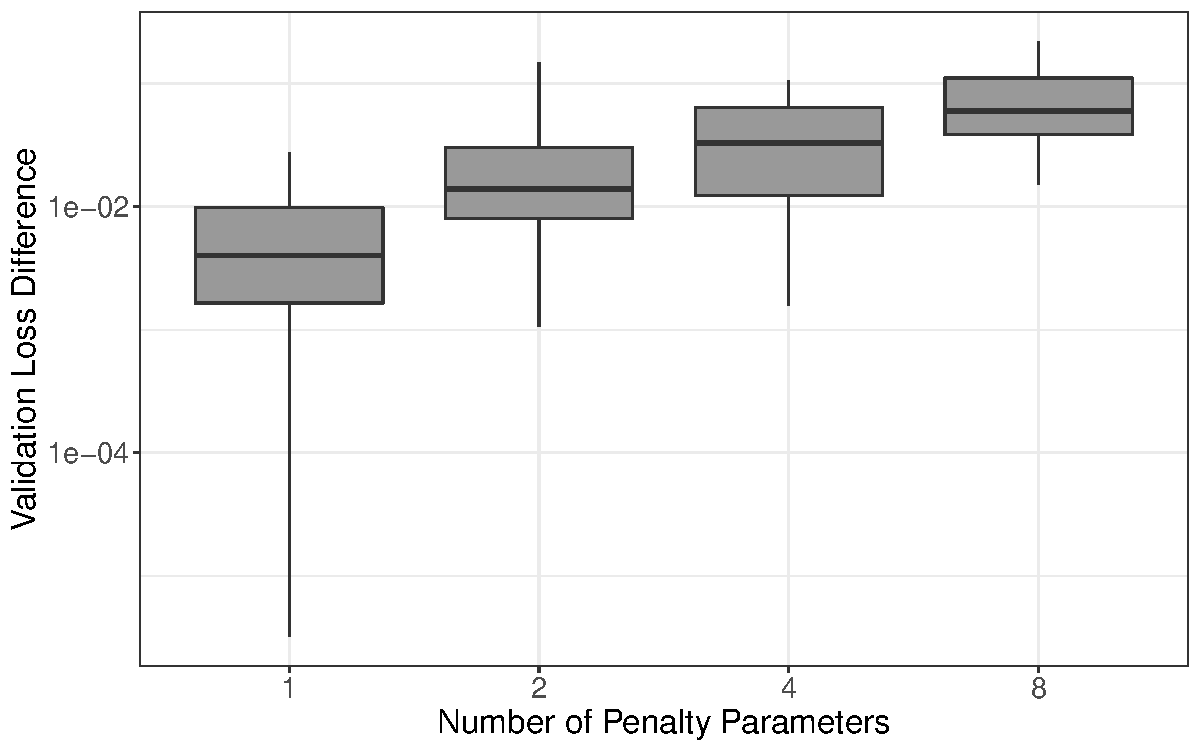
\includegraphics[width=\textwidth]{../../../R/figures/validation_size_loss_diff_homogeneous.pdf}
		\caption{Simulation 1: sum of identical sinusoids}
	\end{subfigure}
	\begin{subfigure}{0.75\textwidth}
		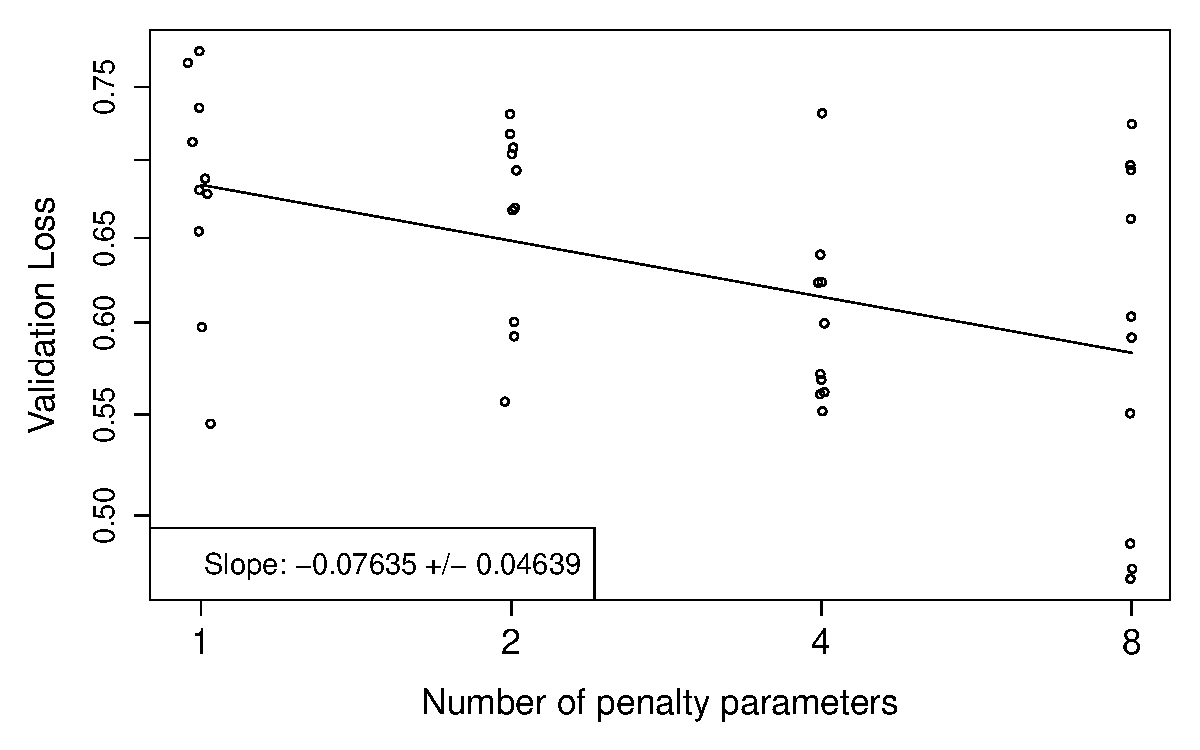
\includegraphics[width=\textwidth]{../../../R/figures/validation_size_loss_heterogeneous.pdf}
		\caption{Simulation 2: sum of sinusoids with increasing frequency}
	\end{subfigure}
	\caption{
		Simulation results for nonparametric additive models as the number of penalty parameters grows.
	}
	\label{fig:simulations}
\end{figure}

\section{Discussion}\label{sec:discussion}

The goal of this paper is to characterize the generalization error of model-estimation procedures that tune multiple hyper-parameters via single training/validation split or $K$-fold cross-validation. 
If the estimated models are Lipschitz with respect to the hyper-parameters, the generalization error of the selected model is upper bounded by a combination of the oracle error, a near-parametric term in the number of hyper-parameters, and a geometric mean of the two.
These results show that if additional hyper-parameters shrink the oracle error term by a sufficient amount, they can improve the performance of the selected model.
In the semi- or non-parametric setting, the error incurred from tuning hyper-parameters is dominated by the oracle error asymptotically; so having many hyper-parameters is unlikely to drastically increase the generalization error of the selected model.
In the parametric setting, the error incurred from tuning hyper-parameters is roughly on the same order as the oracle error; so one should be careful about adding more hyper-parameters, though hyper-parameters are not more ``costly'' than model parameters.


We also considered the special case of penalized regression problems with multiple penalty parameters. In our example of additive univariate models, we show that the estimated models are Lipschitz in the penalty parameters, which means our theoretical results apply. Our results suggest using multiple penalties to induce the desired model characteristics and allowing for many penalty parameters, rather than the usual one or two penalty parameters. Moreover, using recently-developed algorithms for tuning multiple hyper-parameters \citep{bengio2000gradient, foo2008efficient, snoek2012practical}, it is now computationally tractable to test out regularization schemes with many penalty parameters.

One drawback of our theoretical results is that we have assumed it is possible to find the global minimizer of the validation loss. Unfortunately this is computationally intractable since the validation loss is not convex with respect to the hyper-parameters. This problem is exacerbated when there are multiple hyper-parameters since it is computationally infeasible to perform an exhaustive grid-search. We hope to address this question in future research.


%%%%%%%%%%%%%%%%%%%%%%%%%%%%%%%%%%%%%%%%%%%%%%%%%%%%%%%%%%%%%%%%%%%%%%%%%%%%%%%%%%%%%%%%%%%%%%%%%%%%%%%%%%%%%%%%%%%%%%%%%%%%
\vskip 14pt
\noindent {\large\bf Supplementary Materials}

Oracle inequalities for general model-estimation procedures and proofs for all the results are given in the Supplementary Materials.
\par
%%%%%%%%%%%%%%%%%%%%%%%%%%%%%%%%%%%%%%%%%%%%%%%%%%%%%%%%%%%%%%%%%%%%%%%%%%%%%%%%%%%%%%%%%%%%%%%%%%%%%%%%%%%%%%%%%%%%%%%%%%%%
\vskip 14pt
\noindent {\large\bf Acknowledgements}

Jean Feng was supported by NIH grants DP5OD019820 and T32CA206089. Noah Simon was supported by NIH grant DP5OD019820.
\par

\bibliographystyle{unsrtnat}
\bibliography{hyperparam-theory}

\vskip .65cm
\noindent
Jean Feng, Department of Biostatistics, University of Washington
\vskip 2pt
\noindent
E-mail: jeanfeng@u.washington.edu
\vskip 2pt

\noindent
Noah Simon, Department of Biostatistics, University of Washington
\vskip 2pt
\noindent
E-mail: nrsimon@u.washington.edu


\end{document}
